\documentclass{report}
\usepackage[utf8]{inputenc}
\usepackage[a4paper]{geometry}
\usepackage{parskip}
\usepackage[acronym,nonumberlist]{glossaries}
\usepackage{tikz}
\usepackage{url}
\usepackage{pgfplots}
\usepackage{titlesec}
\usepackage{tabularx}
\usepackage{array}
\usepackage{arydshln} %Allow dotted lines in tables
\usepackage{graphicx}
\usepackage{wrapfig}
\pgfplotsset{compat=1.14}

%Changing the Title Format
\titleformat{\chapter}[hang] 
{\normalfont\huge\bfseries}{\thechapter}{1em}{} 
\titlespacing*{\chapter}{0pt}{-50pt}{30pt}

%Adding thick lines for a table
\makeatletter
\newcommand{\thickhline}{%
    \noalign {\ifnum 0=`}\fi \hrule height 1pt
    \futurelet \reserved@a \@xhline
}
\newcolumntype{"}{@{\hskip\tabcolsep\vrule width 1pt\hskip\tabcolsep}}
\makeatother


\makeglossaries

\newacronym{sme}{SME}{small and medium-sized enterprises}
\newacronym{fhtenl}{FHTenL}{Fontys Hogeschool Techniek en Logistiek}
\newacronym{hsnr}{HSNR}{Hochschule Niederrhein}
\newacronym{eu}{EU}{European Union}
\newacronym{mweimh}{MWEIMH NRW}{Ministerium für Wirtschaft, Energie, Industrie, Mittelstand und Handwerk des Landes Nordrhein-Westfalen}
\newacronym{wms}{WMS}{Warehouse Management System}


\author{Lukas Rolle - 2310309}
\title{Project Plan}
\date{\today, Blerick}
\pagenumbering{roman}

\bibliographystyle{abbrv}

\begin{document}
\maketitle
\tableofcontents
\glsaddall

\printglossaries
\listoftables
\listoffigures

\chapter{Introduction}
This document is the project plan for the creation of a demo facility for the LOGwear project.

\section{LOGwear}
LOGwear is a research project that aims to bring wearable to the area of logistics, especially to \gls{sme}. It is a German-Dutch project were multiple parties are cooperating to create results in the research project. Involved in this are two Universities of applied sciences, \gls{fhtenl} in Venlo as the Lead-Partner, Netherlands and \gls{hsnr} in Krefeld, Germany.

Further on there are also multiple partner companies involved in the project namely KLG Europe bv, Helmut Beyers GmbH and imat-uve GmbH. These partner companies are there to give the knowledge about logistics processes, as well as to verify and test the results.

The project is backed within the scope of the INTERREG Deutschland-Nederland initiative. It is backed by the \gls{eu}, \gls{mweimh} and the Provincie Limburg as well.

\section{Demo Facility}
The demo facility that should be created for this project will be a physical environment in which a logistics process can be modelled. This process should then be improved by using a wearable. This will be used as a demonstration area for \gls{sme} to see hands-on if a wearable could be used to improve their own processes. The demo facility will be a proof of concept and not a fully implemented solution that could be directly used at a logistics company and instantly work. %This document will inform the user about the LOGwear project in general and more specifically about the task of creating a demo facility for that project and the boundaries of that task.  The demo facility in this is supposed to show the capabilities of a wearable by displaying it is an actual scenario. What this means is a general logistics process is taken and improved with a wearable and then displayed to interested \gls{sme}. It is supposed to be a proof of concept and not a fully implemented solution that could be directly used at a logistics company and instantly work.
\section{Overview}
In this section the following chapters will be shortly explained. 

The first chapter following this, chapter \ref{cha:scope} is about the scope of the assignment as well as the way of working. The risk management done in the project will be explained in chapter \ref{cha:riskManagement}. The last chapter will be about the existing stakeholders in the project \ref{cha:stakeholders}.
\chapter{Scope}\label{cha:scope}

\section{Inside of the Scope}
\begin{itemize}
	\item Reference Architecture
	\item Prototype Wearable Application
	\item Creation of Physical Demo Area
\end{itemize}

\section{Outside of the Scope}
\begin{itemize}
	\item fully finished product that can be just dropped into a company
	\item Multiple Demo Scenarios
\end{itemize}
\chapter{Risk Management}\label{cha:riskManagement}
Risk management is about identifying risks and finding solutions to problems before they can occur. The list of risks can be found in table \ref{tab:RiskRegister}. The identified risks will increase as the project moves forward. Especially when a decision is made for the wearable and the process. 

\begin{table}[htbp]
\centering
\footnotesize
\resizebox{\textwidth}{!}{
\begin{tabular}{|p{.03\textwidth}|p{.1\textwidth}|p{.2\textwidth}|p{.08\textwidth}|p{.08\textwidth}|p{.15\textwidth}|p{.13\textwidth}|p{.11\textwidth}|}
\hline
\textbf{Nr} & \textbf{Risk Name}                                    & \textbf{Description}                                                                                                      & \textbf{Prob-ability} & \textbf{Impact} & \textbf{Root Cause}                                                                                       & \textbf{Potential Responses}                                              & \textbf{Risk Owner} \\
\hline
1           & Wearable unavailable          & The wearable desired to be used in the demo facility is unavailable.                                                      & Low                  & Medium          & The desired product is a prototype or similar.                                                            & Choosing a different wearable that is already readily available.          & Graduation Student  \\ \hline
2           & Demo Area & A demo area is in mind that could potentially be rented, but that could not be possible.                                  & Medium               & Medium          & The owner of the place does not rent the area.                                                            & Researching possible places where the demo facility could be created.     & Graduation Student  \\ \hline
3           & Unusable wearable             & A wearable is chosen that does not have the capabilities to fulfill the things that were planned with the demo facility.  & Low                  & High            & Too little research done on the wearables, or the researched material was wrong.                          & Altering the demo scenario to accommodate the problems with the wearable. & Graduation Student  \\ \hline
4           & Vocabulary unclear            & The vocabulary used in the logistics branch, especially abbreviations and acronyms might cause problems in communication. & High                 & Low             & The graduation student has too little knowledge of the logistics branch, at the beginning of the project. & Asking questions if a word's or sentence's meaning is not clear.          & Graduation Student. \\ \hline
\end{tabular}
}
\caption{Risk Register}
\label{tab:RiskRegister}
\end{table}

\begin{wrapfigure}{l}{0pt}
	\centering
	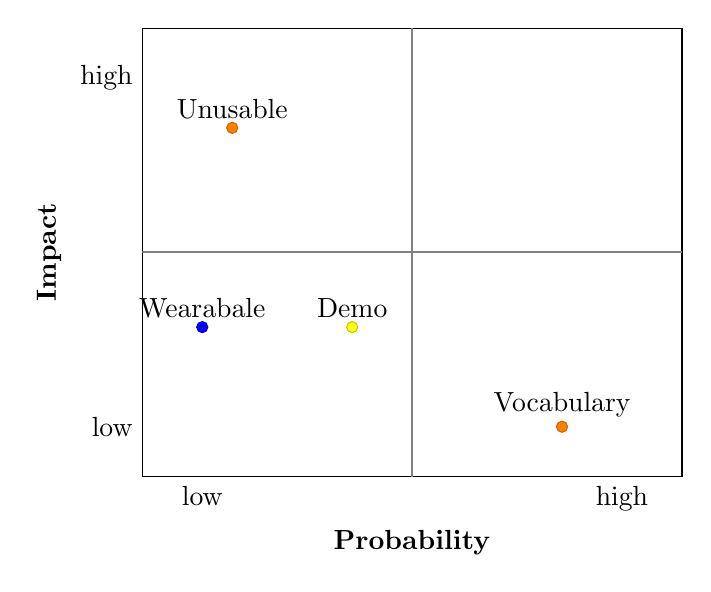
\begin{tikzpicture}
		\begin{axis}[
			scale=1,
			xmin=1,
			xmax=10,
			ymin=1,
			ymax=10,
			xtick,
			ytick,
			extra x ticks={2,9},
  			extra x tick labels={low, high},
  			xtick style={draw = none},
  			extra y ticks={2,9},
  			extra y tick labels={low, high},
			ytick style={draw = none},			
			xlabel=\textbf{Probability},
			ylabel=\textbf{Impact},
			x
			]
			\addplot[
			scatter,
			only marks,
			nodes near coords*={\myvalue},  
			point meta=\thisrow{color},
			visualization depends on={value \thisrow{myvalue} \as \myvalue},
			] table[x=x, y=y]
			{
			x	y	color	myvalue
			2	4	1	Wearabale
			4.5	4	2	Demo
			2.5	8	3	Unusable
			8	2	3	Vocabulary
			0	0 	4
			};
			\addplot[gray,thick, no markers] coordinates {(1,5.5) (10,5.5)};
			\addplot[gray,thick, no markers] coordinates {(5.5,1) (5.5,10)};
		\end{axis}
	\end{tikzpicture}
	\caption{Risk Graph}
	\label{fig:risks}
\end{wrapfigure}

In figure \ref{fig:risks} the risks can be seen in a graph that shows their Probability and Impact again. The color emphasizes the amount of attention a risk should get, in order for the project to continue smoothly.

\chapter{Stakeholders}\label{cha:stakeholders}

\begin{table}[htbp]
\centering
\begin{tabular}{|p{.03\linewidth}|p{.22\linewidth}|p{.12\linewidth}|p{.13\linewidth}|p{.1\linewidth}|p{.1\linewidth}|p{.19\linewidth}|}
\hline
\textbf{Nr} & \textbf{Stakeholder} & \textbf{Company / Institution} & \textbf{Internal / External} & \textbf{Level of Interest} & \textbf{Level of Influence} & \textbf{Potential mgmt strategies} \\ \hline
1  & Employer             & \gls{fhtenl}        & Internal            & Medium            & High               & Keep Satisfied            \\ \hline
2  & Student Workers      & \gls{fhtenl}        & Internal            & Medium            & Low                & Keep Informed             \\ \hline
3  & Pilot Company        & KLG                   & External            & High              & High               & Key Player                \\ \hline
4  & Examiner             & \gls{fhtenl}        & External            & Low               & High               & Keep Satisfied            \\ \hline
5  & Supervising Lecturer & \gls{fhtenl}        & External            & Medium            & Low                & Keep Informed             \\ \hline
6  & Graduation Student   & \gls{fhtenl}        & Internal            & High              & High               & Key Player                \\ \hline
7  & Project Manager      & \gls{fhtenl}        & Internal            & High              & High               & Key Player                \\ \hline
8  & Company Supervisor   & \gls{fhtenl}        & Internal            & High              & High               & Key Player                \\ \hline
9  & Project Team         & \gls{fhtenl}        & Internal            & High              & High               & Key Player                \\ \hline
10 & Partner University   & \gls{hsnr}          & External            & High              & Low                & Keep Informed             \\ \hline
\end{tabular}
\caption{Stakeholder Register}
\label{tab:stakeholder}
\end{table}

\begin{figure}[htbp]
	\centering
	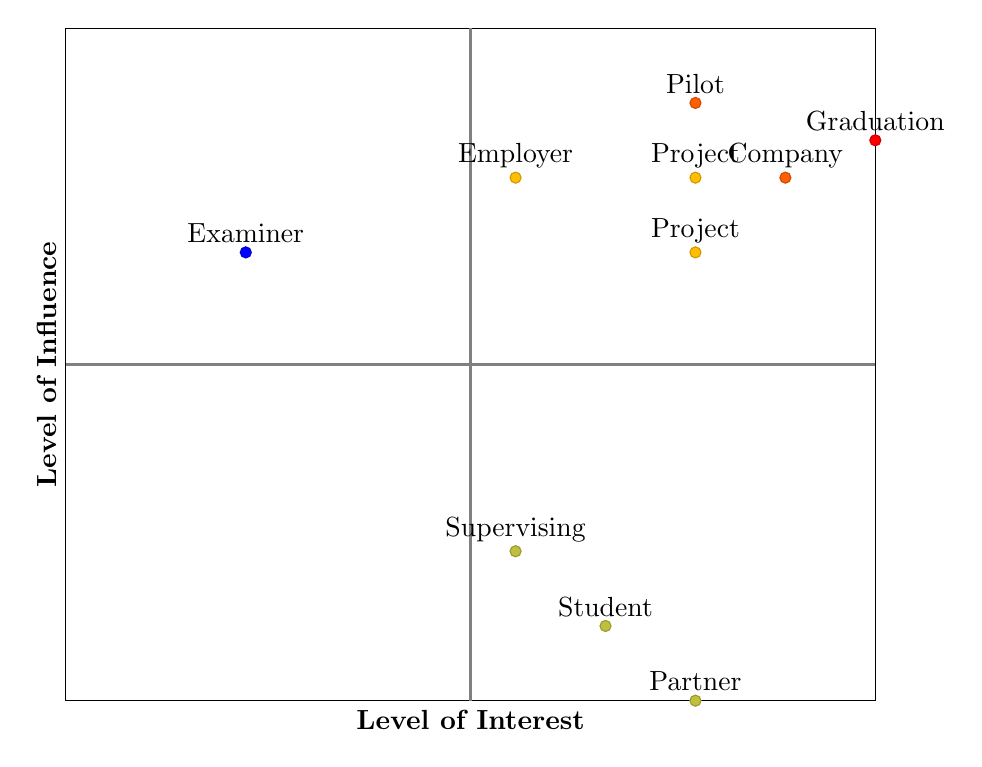
\begin{tikzpicture}
		\begin{axis}[
			scale=1.5,
			xmin=1,
			xmax=10,
			ymin=1,
			ymax=10,
			xtick,
			ytick,
			xlabel=\textbf{Level of Interest},
			ylabel=\textbf{Level of Influence},
			x
			]
			\addplot[
			scatter,
			only marks,
			nodes near coords*={\myvalue},  
			point meta=\thisrow{color},
			visualization depends on={value \thisrow{myvalue} \as \myvalue},
			] table[x=x, y=y]
			{
			x	y	color	myvalue
			6	8	3	Employer
			7	2	2	Student Workers
			8	9	4	Pilot Company 
			3	7	1	Examiner
			6	3	2	Supervising Lecturer
			10	8.5	5	Graduation Student 
			8	8	3	Project Manager 
			9	8	4	Company Supervisor 
			8	7	3	Project Team 
			8	1	2	Partner University
			};
			\addplot[gray,thick, no markers] coordinates {(1,5.5) (10,5.5)};
			\addplot[gray,thick, no markers] coordinates {(5.5,1) (5.5,10)};
		\end{axis}
	\end{tikzpicture}
	\caption{Stakeholder Graph}
	\label{fig:stakeholder}
\end{figure}
\section{Internal Stakeholders}
\section{External Stakeholders}
%\documentclass{report}
\usepackage{parskip}

\begin{document}

\chapter{•}
\begin{verbatim}
 http://www.dhl.com/en/press/releases/releases_2015/logistics/dhl_successfully_tests_augmented_reality_application_in_warehouse.html
DHL's Pilot project has increased productivity by about 25\%.

Show the differences in order picking types
http://www.guoanhong.com/papers/Computer15-OrderPicking.pdf
http://campar.in.tum.de/twiki/pub/Main/BjoernSchwerdtfeger/BjoernsDiss.pdf

\end{verbatim}

\chapter{Initial Analysis}
The process that has been decided on is the Order Picking W3-5. The available Processes were:

\begin{itemize}
	\item Order Picking High Rack
	\item Order Picking W3-5
	\item Goods Receipt and Put away
\end{itemize}

The other two processes were discarded. Order Picking High Rack has been discarded due to the nature of what should be created. A simulation that should model a real environment. Modelling a High Rack and usage of that would be too hard and would take too much time.

Goods Receipt and Put away was another process to be considered, but was discarded. The modelling of it would be problematic due to the time delays in the tasks. Furthermore the process showed less potential for improvements with wearables.

The process has been decided together with the company supervisor.
\chapter{Wearables}
Requirements for Wearables: (from the Order Picking W3-5 process - communications made to the WMS)
\begin{itemize}
	\item (Optionally) Display Order Document
	\item Scan ID
	\item Display Location IDs (Information in General)
	\item Send Confirmations
	\item Confirmation with Signature(?)
\end{itemize}


The goal is to at least fully replace the existing Hand scanner:
Nice to have Features: (Talk with Sobek about these)
\begin{itemize}
	\item Hands-Free (Gesture free ?)
	\item Indoor Navigation
	\item Show exact Location (Display Sector / exact object)
	\item quantity confirmation (?)
	\begin{itemize}
		\item let wearable be a part of the confirmation of the quantity of objects.
		\item an item is picked up
		\item wearable "sees" that
		\item counts on / off screen
		\item if the wrong quantity was counted by the wearable notify the user
	\end{itemize}
	\item Gamification (?) \begin{verbatim} https://youtu.be/9Wv9k_ssLcI?t=173 \end{verbatim}
	\item Route Optimization (?)
\end{itemize}

Wearables:
\begin{itemize}
	\item Daqri Smart Helmet \& Glasses - Only available on contact (Helmet) or as preorder for june (Glasses)
	\item Epson Moverio
	\item Microsoft HoloLens - available
	\item Wuzix (whichever one is available at fontys)
	\item Motorola RS507 - Paired with Motorola WT400 for example? No longer available?
\end{itemize}

\section{HoloLens Risk}
When the HoloLens is getting too hot it closes applications running on the device, what this could mean is, the HoloLens might shut down the application running due to too high processor usage overheating the device.

\chapter{Reference Architecture}
Should the reference architecture be something that is modelled that it could be used by companies without changing a lot of the given code in the reference architecture. 

Or should it be something that is designed and implemented in a way that should fit \textbf{EVERY POSSIBLE} data structure that a company might have with their orders?


\end{document} Has nothing to do in the Project Plan

\bibliography{99-bibliography}


\end{document}
